\section{Ideas}

Choona will be an app that can connect people to music in their location.  Music is something that can be listened to at home, in the office or in public.  We have created an app that allows you to do so.  
\begin{itemize}
  \item \textbf{Home} - 
    In the home, music can be played throughout the home using one medium, but different playlists could be set up for each room, so different family members can listen to the music they want.
  \item \textbf{Office} - 
    In the office, employees can stipulate what music they wish to listen to.  This can be via the main system where the music is just something heard in the background.  There is the option of using a mobile device to play the music privately where the user can plug in their earphones, listen to the music and zone-out the office background.  
  \item \textbf{Surrounding area} - 
    When we speak of your surrounding area, we are talking about restaurants, bars, coffee shops retailers and more. In this type of scenario, users can queue songs they want to hear.  They can also interact by liking/unliking a song choice.  For businesses, this could be a way to enhance a customers visit and entice them to come back again. The potential for this is huge because as well as homes, surrounding area and the office, it could be rolled out in hotels, library's and potentially public transport creating a large user base.
\end{itemize}
The app could allow the user to suggest songs they wish to be played either right away or at a specified time.  The thought of having a song played at a particular time could almost be used an alarm clock for e.g. user could wish to play a song at 5pm which would subconsciously indicate the end of their working day or lunchbreak etc.\\\\
The system infrastructure is going to be built upon four main layers, as illustrated in Figure \ref{sys-architecture}:
\begin{itemize}
  \item \textbf{Source} - 
    When we listen to music, we need to take it from a source.  There are two different types of sources we need to consider for this project.  First of all there are the virtual sources.  Virtual sources are your software streaming packages such as `Spotify', `Youtube', `Google Play Music' etc.  At the moment, we will not consider iTunes as a virtual source because iTunes music needs to be purchased before streaming whereas with sources such as Spotify, a subscription to the service only needs to be purchased.  Secondly, there are the physical sources.  These include iPods, MP3 players and other hardware devices where the songs are stored as data files.  

    We want to make sure that the app is not just configured for one music source, but a host of sources leading to a larger audience and a greater variety of music.  As all these sources are different, we shall need to have adaptors in place where the data is converted into the same format so it can be understood by our service application making it available to many sources and hardwares.  
  \item \textbf{Service Layer} - 
    We shall have a service layer that serves our app, provides us with value-added service such as song queueing and gives us access to our data sources.   It will consist of a database that in essence will contain all the data we need to access the different music sources, communication between the API's.  
  \item \textbf{Access APIs} - 
    We will need to have certain API's in place that accomplish specific tasks.  We will need an API that is responsible for streaming the right music from it's source, an API that takes care of the control aspect of the project e.g. which songs will play next, denoting the available songs etc.  A management API will generally manage the whole system in terms of access rights etc. 
  \item \textbf{Client Layer} - 
    Finally we have the client layer which consists of the app and the hardware that outputs the music.  The UI (User Interface) design must be 100\% accurate if we are to gain a huge user base.  The app makes it easy for a user to carry out a task and that it is intuitive in the sense that it's not hard to learn.  The design needs to be consistent and minimilistic and finally bug free.
    When it comes to the output (i.e. speakers), adaptors may need to be in place so that the app can communicate with it.  However, in the case of WiFi speakers, we should be able to stream the music wirelessly to the speakers.
\end{itemize}

There is potential to eventually integrate NFC within this app.  Something that could be considered would be placing NFC tags around a shop, tables in a coffee shop etc. the playlist for that location would autmatically pop up in the app. This makes finding the playlist much simplier for the user. 

\begin{minipage}{\linewidth}
  \centering
  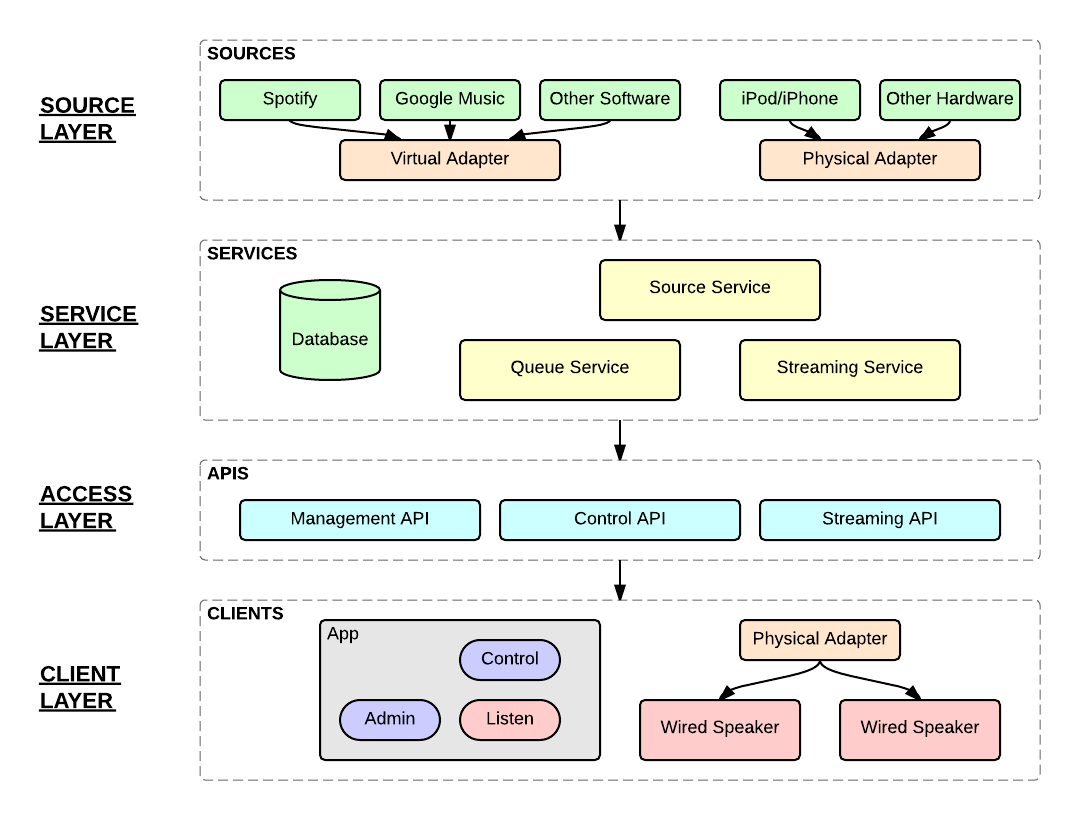
\includegraphics[width=1\textwidth]{./img/sys-architecture.png}
  \captionof{figure}{Concept system architecture}\label{sys-architecture}
\end{minipage}